\section{Proocessing Data}
In the past two weeks,we have learned how to process data with code and draw pictures with paraview.
\subsection{Extract Data}
\begin{figure}[htbp]
\centering
    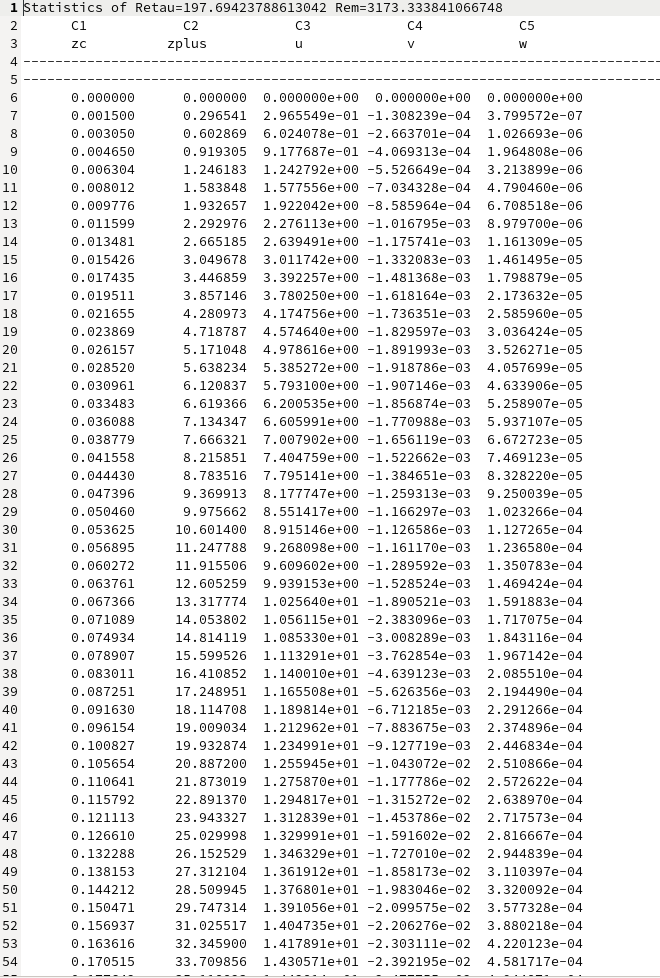
\includegraphics[width=0.35\textwidth]{src/Screenshot from 2020-12-19 14-49-07.png}
\caption{Velocity in diffeent directios}
\label{pd}
\end{figure}

\subsection{Draw pictures}
\begin{figure}[htbp]
\centering
    \subfigure[Distribution of velocity u in XZ section]{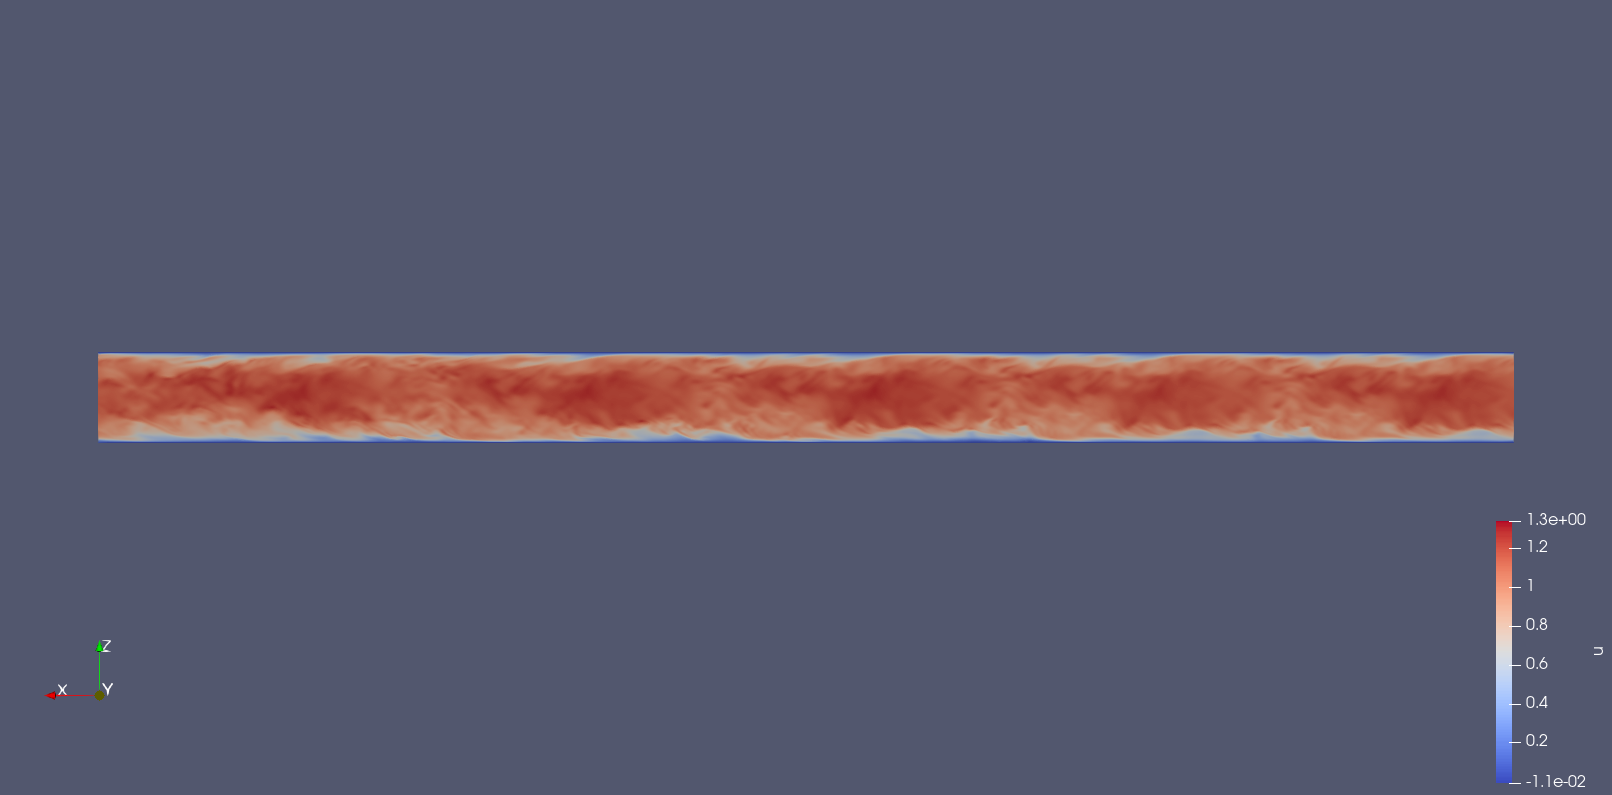
\includegraphics[width=0.8\textwidth]{src/u1.png}}
    \subfigure[Distribution of velocity u in YZ section]{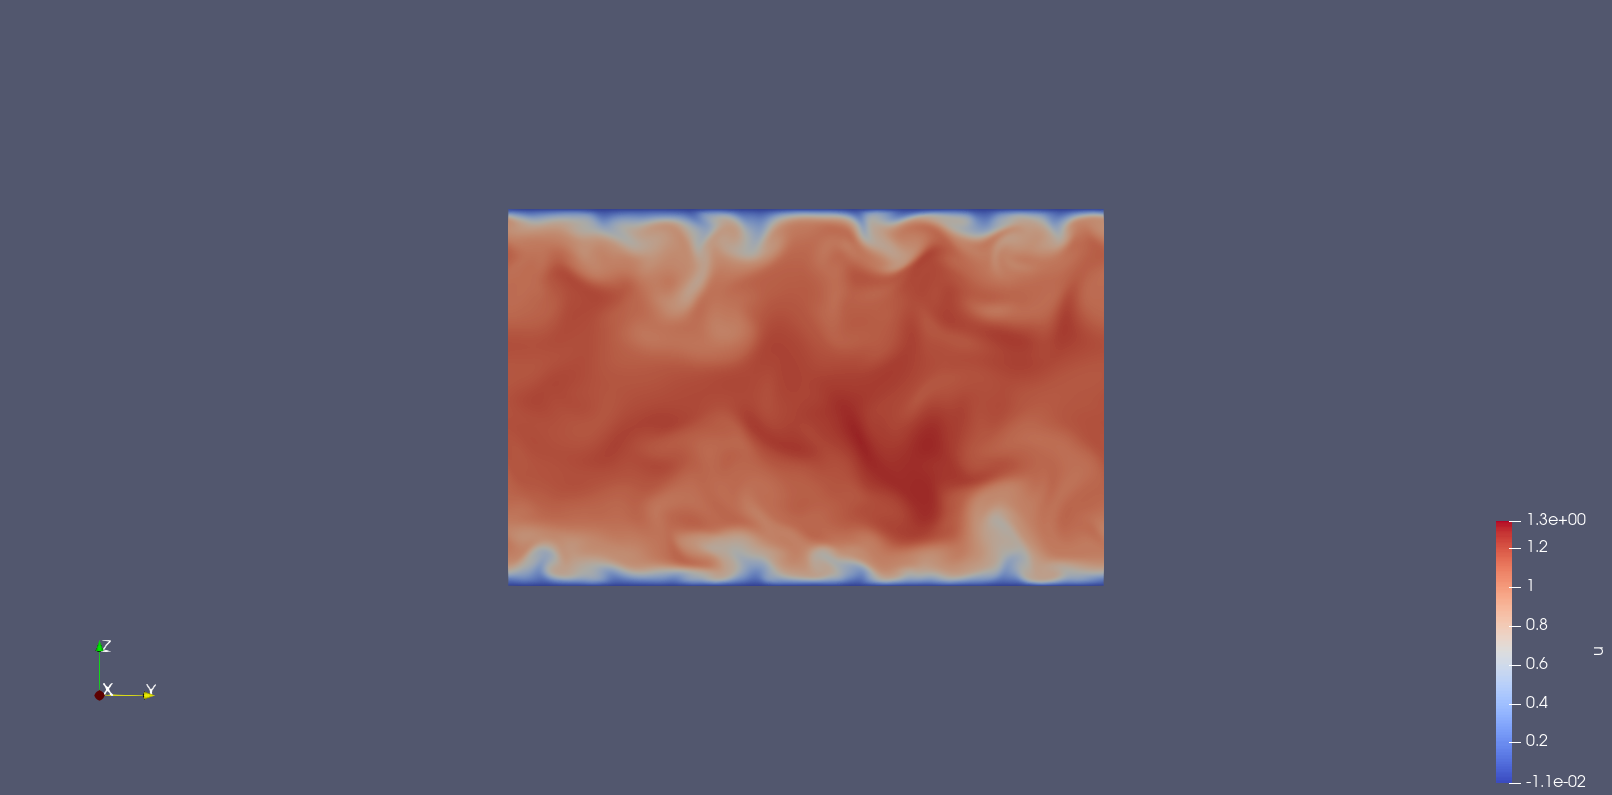
\includegraphics[width=0.8\textwidth]{src/u.png}}
\caption{Distribution of velocity u in different sections}
\label{pd}
\end{figure}
